\PassOptionsToPackage{table}{xcolor}
\documentclass[aspectratio=169]{beamer}
\mode<presentation>
{
  \usetheme{Madrid}
  \usecolortheme{default}
  \usefonttheme{serif}
  \setbeamertemplate{navigation symbols}{}
  \setbeamertemplate{caption}[numbered]
} 
\usepackage[english]{babel}
\usepackage[utf8x]{inputenc}
\usepackage[version=3]{mhchem}
\usepackage{pgfpages}
\usepackage{algorithm,algpseudocode}
\usepackage{amsmath}
\usepackage{csquotes}
\usepackage{soul}
\usepackage {enumerate}
\usepackage{amsthm}
\usepackage{tikz}
\usepackage[T1]{fontenc}
\usepackage{mathtools}
\usepackage{caption}
\usepackage{subcaption}
\newcommand {\eps} {\varepsilon}
\newcommand{\highlight}[1]{%
  \colorbox{red!50}{$\displaystyle#1$}}
\newcommand\hcancel[2][black]{\setbox0=\hbox{$#2$}%
\rlap{\raisebox{.45\ht0}{\textcolor{#1}{\rule{\wd0}{1pt}}}}#2} 
\title[Strassens Algorithmus]{Strassens Algorithmus \\ für die Matrixmultiplikation}
\author{Bashar Khoulani}
\institute[]{Universität Kassel}
\date{\today}

\begin{document}

\begin{frame}
    \titlepage
\end{frame}

\section{Einführung}
\begin{frame}{Einführung --- Anwendungen}
\uncover<+-> {
Matrixmultiplikation in der Anwendung:
\begin{itemize}[<+->]
\item Lösung von linearen Gleichungssystemen
\item Transitiven Abschluss eines Graphen berechnen
\item Inverse und Determinante einer Matrix
\item Kürzeste Pfade in einem Graphen finden
\end{itemize}
}
\end{frame}

\begin{frame}{Einführung --- Matrixmultiplikation}
\uncover<+->{
Matrixmultiplikation wie aus der linearen Algebra bekannt:
}
\uncover<+-> {
\[
\cdot: R^{n\times l} \times R^{l\times m} \rightarrow R^{n\times m}, (A, B) \mapsto C = A \cdot B
\]
\[\text{ mit } 
c_{ij} = \sum_{k=1}^{l} a_{ik}b_{kj} \text{, für }i = 1, \dots, n \text{ und }j = 1, \dots, m
\]
}
\uncover<+-> {
Beispiel: $\cdot: \mathbb{Z}^{n\times l} \times \mathbb{Z}^{l\times m} \rightarrow \mathbb{Z}^{n\times m}, (A, B) \mapsto C = A \cdot B$
\alt<3>{
\[
    \begin{pmatrix}
    \; 1 & 2 & 3 \text{ }\\
    \; 4 & 5 & 6 \text{ }\\
    \; 7 & 8 & 9 \text{ }
    \end{pmatrix} \cdot 
    \begin{pmatrix}
    \; 1 & 2 \text{ }\\
    \; 3 & 4 \text{ }\\
    \; 5 & 6 \text{ }
    \end{pmatrix} =
    \begin{pmatrix}
    \; \phantom{22} & \; \phantom{28} \text{ } \\
    \; \phantom{49} & \; \phantom{64} \text{ } \\
    \; \phantom{76} & \; \phantom{100} \text{ } 
    \end{pmatrix} 
\]}{
\alt<4>{
\[
    \left(\begin{array}{ccc}
    \rowcolor{red!20}
    1 & 2 & 3\\
    4 & 5 & 6\\
    7 & 8 & 9
    \end{array}\right) \cdot 
    \left(\begin{array}{>{\columncolor{blue!20}}cc}
    1 & 2\\
    3 & 4\\
    5 & 6
    \end{array}\right) =
    \left(\begin{array}{cccc}
    \cellcolor{green!10} 22 & \phantom{28} \\
    \phantom{49} & \phantom{64} \\
    \phantom{76} & \phantom{100} 
    \end{array}\right) 
\]}{
\alt<5>{
\[
    \left(\begin{array}{ccc}
    \rowcolor{red!20}
    1 & 2 & 3\\
    4 & 5 & 6\\
    7 & 8 & 9
    \end{array}\right) \cdot 
    \left(\begin{array}{c>{\columncolor{blue!20}}c}
    1 & 2\\
    3 & 4\\
    5 & 6
    \end{array}\right) =
    \left(\begin{array}{cccc}
    22 & \cellcolor{green!10} 28 \\
    \phantom{49} & \phantom{64} \\
    \phantom{76} & \phantom{100} 
    \end{array}\right) 
\]}{
\alt<6>{
\[
    \left(\begin{array}{ccc}
    1 & 2 & 3\\
    \rowcolor{red!20}
    4 & 5 & 6\\
    7 & 8 & 9
    \end{array}\right) \cdot 
    \left(\begin{array}{>{\columncolor{blue!20}}cc}
    1 & 2\\
    3 & 4\\
    5 & 6
    \end{array}\right) =
    \left(\begin{array}{cccc}
    22 & 28 \\
    \cellcolor{green!10} 49 & \phantom{64} \\
    \phantom{76} & \phantom{100} 
    \end{array}\right) 
\]
}{
\alt<7>{
\[
    \left(\begin{array}{ccc}
    1 & 2 & 3\\
    \rowcolor{red!20}
    4 & 5 & 6\\
    7 & 8 & 9
    \end{array}\right) \cdot 
    \left(\begin{array}{c>{\columncolor{blue!20}}c}
    1 & 2\\
    3 & 4\\
    5 & 6
    \end{array}\right) =
    \left(\begin{array}{cccc}
    22 & 28 \\
    49 & \cellcolor{green!10} 64 \\
    \phantom{76} & \phantom{100} 
    \end{array}\right) 
\]}{
\alt<8>{
\[
    \left(\begin{array}{ccc}
    1 & 2 & 3\\
    4 & 5 & 6\\
    \rowcolor{red!20}
    7 & 8 & 9
    \end{array}\right) \cdot 
    \left(\begin{array}{>{\columncolor{blue!20}}cc}
    1 & 2\\
    3 & 4\\
    5 & 6
    \end{array}\right) =
    \left(\begin{array}{cc}
    22 & 28 \\
    49 & 64 \\
    \cellcolor{green!10} 76 & \phantom{100} 
    \end{array}\right) 
\]}{
\[
    \left(\begin{array}{ccc}
    1 & 2 & 3\\
    4 & 5 & 6\\
    \rowcolor{red!20}
    7 & 8 & 9
    \end{array}\right) \cdot 
    \left(\begin{array}{c>{\columncolor{blue!20}}c}
    1 & 2\\
    3 & 4\\
    5 & 6
    \end{array}\right) =
    \left(\begin{array}{cc}
    22 & 28 \\
    49 & 64 \\
    76 & \cellcolor{green!10} 100 
    \end{array}\right) 
\]}}}}}}}

\pause[9]
\end{frame}

\begin{frame}{Behandelnde Algorithmen}
    In diesem Vortrag zu behandelnde Algorithmen:
    \begin{itemize}
        \item \st{Der "naive" Algorithmus}
        \begin{itemize}
            \item[--] $\Theta(n^3)$
        \end{itemize}
    \end{itemize}
\end{frame}

\begin{frame}{Einführung --- Master-Theorem}
    \begin{theorem}[Master-Theorem]
    Seien $a \geq 1$ und $b > 1$ Konstanten.
    Sei $ f: \mathbb{R}^{\geq 0} \rightarrow \mathbb{R}^{\geq 0}$ eine Funktion, und sei $T : \mathbb{N} \rightarrow \mathbb{N}$ durch die folgende Rekursion definiert:
    \[
        T(n) = a \cdot T \left(\frac{n}{b}\right) + f(n)
    \]
    Dann gilt:
    \begin{itemize}
        
        \item Wenn $f(n) \in \mathcal{O}(n^{log_b\;a-\eps}) $ für ein $\eps$ $>$ $0$, dann gilt $T(n) \in \Theta(n^{log_b\;a})$.
        \tikz\node[opacity=0.25, align=left, inner xsep=0pt] {
        \parbox[t]{\linewidth}{
            \item Wenn $f(n) \in \Theta(n^{log_b\;a})$, dann gilt $T(n) \in \Theta(n^{log_b\;a}\;\lg\,n)$.
        }};
        \tikz\node[opacity=0.25, align=left, inner xsep=0pt] {
        \parbox[t]{\linewidth}{
            \item Wenn $f(n) \in \Omega(n^{log_b\;a+\eps}) $ für ein $\eps$ $>$ $0$ und $a\,f\left(\frac{n}{b}\right) \leq c\,f(n)$ für ein $c$ $<$ $1$ und hinreichend großen n, dann gilt $T(n) \in \Theta(f(n))$.
        }};
        
    \end{itemize}
    \end{theorem}
\end{frame}

\begin{frame}{Divide-And-Conquer --- Einführung}
    \uncover<+->{
        Annahme: $A$, $B$ und $C$ sind $2^k \times 2^k$-Matrizen \\
        \bigskip
}
    \uncover<+->{Partitioniere $A$, $B$ und $C$ für $k \geq 1$ wie in \ref{partition}.  \\
        \bigskip
        Dann gilt für das Produkt $A\cdot B = C$:
        \begin{equation}
            \left(\begin{array}{cc}
                A_{11} & A_{12} \\
                A_{21} & A_{22} 
            \end{array}\right) \cdot
            \left(\begin{array}{cc}
                B_{11} & B_{12} \\
                B_{21} & B_{22} 
            \end{array}\right) =
            \left(\begin{array}{cc}
                C_{11} & C_{12} \\
                C_{21} & C_{22} 
            \end{array}\right)
        \label{partition}
        \end{equation}
    }
    \uncover<+->{Mit
    \begin{equation}
        C_{11} = A_{11} \cdot B_{11} + A_{12} \cdot B_{21}
    \end{equation}
    \begin{equation}
        C_{12} = A_{11} \cdot B_{12} + A_{12} \cdot B_{22}
    \end{equation}
    \begin{equation}
        C_{21} = A_{21} \cdot B_{11} + A_{22} \cdot B_{21}
    \end{equation}
    \begin{equation}
        C_{22} = A_{21} \cdot B_{12} + A_{22} \cdot B_{22}
    \end{equation}
    }
\end{frame}

\begin{frame}{Divide-And-Conquer --- Analyse}
    Aufgestellte Rekurrenzgleichung:
    \[ T(n) =  \begin{cases*}
                    \Theta(1) & \text{n $\leq$ 1,} \\
                    8 \cdot T\left(\frac{n}{2}\right) + \Theta(n^2) & \text{n $>$ 1} 
                \end{cases*}
    \]
    \onslide<2->{
    \begin{itemize}
        \item  Wenn $f(n) \in \mathcal{O}(n^{log_b\;a-\eps}) $ für ein $\eps$ $>$ $0$, dann gilt $T(n) \in \Theta(n^{log_b\;a})$
    \end{itemize}
    \begin{align*}
        a = 8,\;b = 2,\;f(n) \in \Theta(n^{2}) & \onslide<3->{\rightsquigarrow n^{log_b\;a} = n^{log_2\;8} = n^3 \\}
        \onslide<4->{& \rightsquigarrow f(n) \in \mathcal{O}(n^{3-\eps}) \text{ mit } \eps = 1\\}
        \onslide<5->{& \rightsquigarrow T(n) \in \Theta(n^{log_b\;a}) = \Theta(n^{log_2\;8}) = \Theta(n^{3})}
    \end{align*}
    \onslide<6->{$\rightarrow$ Keine Verbesserung}
    }
\end{frame}

\begin{frame}{Behandelnde Algorithmen}
    In diesem Vortrag zu behandelnde Algorithmen:
    \begin{itemize}
        \item \st{Der "naive" Algorithmus}
        \begin{itemize}
            \item $\Theta(n^3)$
        \end{itemize}
        \item \st{Divide-And-Conquer-Algorithmus}
        \begin{itemize}
            \item $\Theta(n^3)$
        \end{itemize}
    \end{itemize}
\end{frame}




\section{Strassens Algorithmus}

\begin{frame}{Strassens Algorithmus --- Intuition}
    Bewusste Kompromisse:
    \bigskip
    \begin{itemize}
        \item Reduzierung der Multiplikationen 
        \item Erhöhung der Additionen
    \end{itemize}

    \bigskip
    \bigskip
    \uncover<2-> {
    
    Beispiel:
    \begin{center}
         $x^2 - y^2 = x \cdot x - y \cdot y = (x - y) \cdot (x + y)$ 
    \end{center}
   
    }
    
    
\end{frame}


\begin{frame}{Strassens Algorithmus --- Einführung}
    \onslide<1-> {Annahme: $A$, $B$ und $C$ sind $2^k \times 2^k$-Matrizen \\}
    \onslide<2-> {Partitioniere $A$, $B$ und $C$ wie in DAC, dann ist mit:}
    \begin{align*} 
        \onslide<3-> {P_{1} = A_{11} \cdot \left(B_{12} - B_{22}\right) \; \; \; \; & P_{2} = B_{22} \cdot \left(A_{11} + A_{12}\right) \\}
        \onslide<4-> {P_{3} = B_{11} \cdot \left(A_{21} + A_{22}\right) \; \; \; \; & P_{4} = A_{22} \cdot \left(B_{21} - B_{11}\right) \\}
        \onslide<5-> {P_{5} = \left(B_{11} + B_{22}\right) \cdot \left(A_{11} + A_{22}\right) \; \; \; \; & P_{6} = \left(B_{21} + B_{22}\right) \cdot \left(A_{12} - A_{22}\right) \\}
        \onslide<6-> {P_{7} = \left(A_{11} - A_{21}\right) \cdot \left(B_{11} + B_{12}\right) \; \; \; \; &}
    \end{align*}
    \onslide<7-> {
    \begin{align*}
            C =
            \left(\begin{array}{cc}
                P_{4} + P_{5} + P_{6} - P_{2} & P_{1} + P_{2} \\
                P_{3} + P_{4} & P_{1} + P_{5} - P_{3} - P_{7} 
            \end{array}\right)
        \end{align*}
    }
\end{frame}


\begin{frame}{Strassens Algorithmus --- Endergebnis}
\uncover<+-> {
\alt<1> {
Behauptung: Es gilt $A\cdot B = C$:

\bigskip
Beweis:
        \begin{align*}
            A\cdot B =
            \left(\begin{array}{cc}
                P_{4} + P_{5} + P_{6} - P_{2} & P_{1} + P_{2} \\
                P_{3} + P_{4} & P_{1} + P_{5} - P_{3} - P_{7} 
            \end{array}\right)
        \end{align*}
        } {
        \alt<2> {
            \begin{align*}
                A\cdot B =
                \left(\begin{array}{cc}
                    \cellcolor{green!10} P_{4} + P_{5} + P_{6} - P_{2} & P_{1} + P_{2} \\
                    P_{3} + P_{4} & P_{1} + P_{5} - P_{3} - P_{7} 
                \end{array}\right)
            \end{align*}
        
            \begin{align*}
                \highlight{A_{22} \cdot B_{21}} - A_{22} \cdot B_{11} + A_{11} \cdot B_{11} + A_{11} \cdot B_{22} \\ 
                + A_{22} \cdot B_{11} + A_{22} \cdot B_{22} + A_{12} \cdot B_{21} + A_{12} \cdot B_{22} \\ 
                - \highlight{A_{22} \cdot B_{21}} - A_{22} \cdot B_{22} - A_{11} \cdot B_{22} - A_{12} \cdot B_{22} \\
                \;= &\;A_{11} \cdot B_{11} + A_{12} \cdot B_{21}
            \end{align*}} {
        \alt<3> {
            \begin{align*}
                A\cdot B =
                \left(\begin{array}{cc}
                    \cellcolor{green!10} P_{4} + P_{5} + P_{6} - P_{2} & P_{1} + P_{2} \\
                    P_{3} + P_{4} & P_{1} + P_{5} - P_{3} - P_{7} 
                \end{array}\right)
            \end{align*}
            
            \begin{align*}
                \hcancel[red]{A_{22} \cdot B_{21}} - \highlight{A_{22} \cdot B_{11}} + A_{11} \cdot B_{11} + A_{11} \cdot B_{22} & \\ 
                + \highlight{A_{22} \cdot B_{11}} + A_{22} \cdot B_{22} + A_{12} \cdot B_{21} + A_{12} \cdot B_{22} & \\ 
                - \hcancel[red]{A_{22} \cdot B_{21}} - A_{22} \cdot B_{22} - A_{11} \cdot B_{22} - A_{12} \cdot B_{22} & \\
                \;= &\;A_{11} \cdot B_{11} + A_{12} \cdot B_{21}
            \end{align*}}{
            \alt<4>{
                \begin{align*}
                    A\cdot B =
                    \left(\begin{array}{cc}
                        \cellcolor{green!10} P_{4} + P_{5} + P_{6} - P_{2} & P_{1} + P_{2} \\
                        P_{3} + P_{4} & P_{1} + P_{5} - P_{3} - P_{7} 
                    \end{array}\right)
                \end{align*}
                \begin{align*}
                    \hcancel[red]{A_{22} \cdot B_{21}} - \hcancel[red]{A_{22} \cdot B_{11}} + A_{11} \cdot B_{11} + \highlight{A_{11} \cdot B_{22}} & \\ 
                    + \hcancel[red]{A_{22} \cdot B_{11}} + A_{22} \cdot B_{22} + A_{12} \cdot B_{21} + A_{12} \cdot B_{22} & \\ 
                    - \hcancel[red]{A_{22} \cdot B_{21}} - A_{22} \cdot B_{22} - \highlight{A_{11} \cdot B_{22}} - A_{12} \cdot B_{22} & \\
                    \;= &\;A_{11} \cdot B_{11} + A_{12} \cdot B_{21}
                \end{align*}}{
            \alt<5>{
                \begin{align*}
                    A\cdot B =
                    \left(\begin{array}{cc}
                        \cellcolor{green!10} P_{4} + P_{5} + P_{6} - P_{2} & P_{1} + P_{2} \\
                        P_{3} + P_{4} & P_{1} + P_{5} - P_{3} - P_{7} 
                    \end{array}\right)
                \end{align*}
                \begin{align*}
                    \hcancel[red]{A_{22} \cdot B_{21}} - \hcancel[red]{A_{22} \cdot B_{11}} + A_{11} \cdot B_{11} + \hcancel[red]{A_{11} \cdot B_{22}} & \\ 
                    + \hcancel[red]{A_{22} \cdot B_{11}} + \highlight{A_{22} \cdot B_{22}} + A_{12} \cdot B_{21} + A_{12} \cdot B_{22} & \\ 
                    - \hcancel[red]{A_{22} \cdot B_{21}} - \highlight{A_{22} \cdot B_{22}} - \hcancel[red]{A_{11} \cdot B_{22}} - A_{12} \cdot B_{22} & \\
                    \;= &\;A_{11} \cdot B_{11} + A_{12} \cdot B_{21}
                \end{align*}} {
                \alt<6>{
                    \begin{align*}
                        A\cdot B =
                        \left(\begin{array}{cc}
                            \cellcolor{green!10} P_{4} + P_{5} + P_{6} - P_{2} & P_{1} + P_{2} \\
                            P_{3} + P_{4} & P_{1} + P_{5} - P_{3} - P_{7} 
                        \end{array}\right)
                    \end{align*}
                    \begin{align*}
                        \hcancel[red]{A_{22} \cdot B_{21}} - \hcancel[red]{A_{22} \cdot B_{11}} + A_{11} \cdot B_{11} + \hcancel[red]{A_{11} \cdot B_{22}} & \\ 
                        + \hcancel[red]{A_{22} \cdot B_{11}} + \hcancel[red]{A_{22} \cdot B_{22}} + A_{12} \cdot B_{21} + \highlight{A_{12} \cdot B_{22}} & \\ 
                        - \hcancel[red]{A_{22} \cdot B_{21}} - \hcancel[red]{A_{22} \cdot B_{22}} - \hcancel[red]{A_{11} \cdot B_{22}} - \highlight{A_{12} \cdot B_{22}} & \\
                        \;= &\;A_{11} \cdot B_{11} + A_{12} \cdot B_{21}
                    \end{align*}} { 
                \alt<7> {\begin{align*}
                    A\cdot B =
                    \left(\begin{array}{cc}
                        \cellcolor{green!10} P_{4} + P_{5} + P_{6} - P_{2} & P_{1} + P_{2} \\
                        P_{3} + P_{4} & P_{1} + P_{5} - P_{3} - P_{7} 
                    \end{array}\right)
                \end{align*}
                \begin{align*}
                    \hcancel[red]{A_{22} \cdot B_{21}} - \hcancel[red]{A_{22} \cdot B_{11}} + A_{11} \cdot B_{11} + \hcancel[red]{A_{11} \cdot B_{22}} & \\ 
                    + \hcancel[red]{A_{22} \cdot B_{11}} + \hcancel[red]{A_{22} \cdot B_{22}} + A_{12} \cdot B_{21} + \hcancel[red]{A_{12} \cdot B_{22}} & \\ 
                    - \hcancel[red]{A_{22} \cdot B_{21}} - \hcancel[red]{A_{22} \cdot B_{22}} - \hcancel[red]{A_{11} \cdot B_{22}} - \hcancel[red]{A_{12} \cdot B_{22}} & \\
                    \;= &\;A_{11} \cdot B_{11} + A_{12} \cdot B_{21}
                \end{align*}}{\alt<8>{
                \begin{align*}
                    A\cdot B =
                    \left(\begin{array}{cc}
                         P_{4} + P_{5} + P_{6} - P_{2} & \cellcolor{green!10} P_{1} + P_{2} \\
                        P_{3} + P_{4} & P_{1} + P_{5} - P_{3} - P_{7} 
                    \end{array}\right)
                \end{align*}}{
                \alt<9>{\begin{align*}
                    A\cdot B =
                    \left(\begin{array}{cc}
                        P_{4} + P_{5} + P_{6} - P_{2} & \cellcolor{green!10}  P_{1} + P_{2} \\
                        P_{3} + P_{4} & P_{1} + P_{5} - P_{3} - P_{7} 
                    \end{array}\right)
                \end{align*}
                \begin{align*}
                A_{11} \cdot B_{12} - \highlight{A_{11} \cdot B_{22}} \\ 
                + \highlight{A_{11} \cdot B_{22}} + A_{12} \cdot B_{22} \\ 
                \;= &\;A_{11} \cdot B_{12} + A_{12} \cdot B_{22}
                \end{align*}}{
                \alt<10> {\begin{align*}
                    A\cdot B =
                    \left(\begin{array}{cc}
                        P_{4} + P_{5} + P_{6} - P_{2} & \cellcolor{green!10}  P_{1} + P_{2} \\
                        P_{3} + P_{4} & P_{1} + P_{5} - P_{3} - P_{7} 
                    \end{array}\right)
                \end{align*}
                \begin{align*}
                A_{11} \cdot B_{12} - \hcancel[red]{A_{11} \cdot B_{22}} \\ 
                + \hcancel[red]{A_{11} \cdot B_{22}} + A_{12} \cdot B_{22} \\ 
                \;= &\;A_{11} \cdot B_{12} + A_{12} \cdot B_{22}
                \end{align*}}{
                \alt<11>{\begin{align*}
                    A\cdot B =
                    \left(\begin{array}{cc}
                        P_{4} + P_{5} + P_{6} - P_{2} &   P_{1} + P_{2} \\
                        \cellcolor{green!10} P_{3} + P_{4} & P_{1} + P_{5} - P_{3} - P_{7} 
                    \end{array}\right)
                \end{align*}
                \begin{align*}
                A_{21} \cdot B_{11} + \highlight{A_{22} \cdot B_{11}} \\ 
                + A_{22} \cdot B_{21} - \highlight{A_{22} \cdot B_{11}} \\ 
                \;= &\;A_{21} \cdot B_{11} + A_{22} \cdot B_{21}
                \end{align*}}{\alt<12>{\begin{align*}
                    A\cdot B =
                    \left(\begin{array}{cc}
                        P_{4} + P_{5} + P_{6} - P_{2} &   P_{1} + P_{2} \\
                        \cellcolor{green!10} P_{3} + P_{4} & P_{1} + P_{5} - P_{3} - P_{7} 
                    \end{array}\right)
                \end{align*}
                \begin{align*}
                A_{21} \cdot B_{11} + \hcancel[red]{A_{22} \cdot B_{11}} \\ 
                + A_{22} \cdot B_{21} - \hcancel[red]{A_{22} \cdot B_{11}} \\ 
                \;= &\;A_{21} \cdot B_{11} + A_{22} \cdot B_{21}
                \end{align*}}{\alt<13>{\begin{align*}
                A\cdot B =
                \left(\begin{array}{cc}
                    P_{4} + P_{5} + P_{6} - P_{2} & P_{1} + P_{2} \\
                    P_{3} + P_{4} & \cellcolor{green!10} P_{1} + P_{5} - P_{3} - P_{7} 
                \end{array}\right)
            \end{align*}
        
            \begin{align*}
                \highlight{A_{11} \cdot B_{12}} - A_{11} \cdot B_{22} + A_{11} \cdot B_{11} + A_{11} \cdot B_{22} \\ 
                + A_{22} \cdot B_{11} + A_{22} \cdot B_{22} - A_{21} \cdot B_{11} - A_{22} \cdot B_{11} \\ 
                - A_{11} \cdot B_{11} - \highlight{A_{11} \cdot B_{12}} + A_{21} \cdot B_{11} + A_{21} \cdot B_{12} \\
                \;= &\;A_{21} \cdot B_{12} + A_{22} \cdot B_{22}
            \end{align*}}{
            \alt<14>{
                \begin{align*}
                    A\cdot B =
                    \left(\begin{array}{cc}
                        P_{4} + P_{5} + P_{6} - P_{2} & P_{1} + P_{2} \\
                        P_{3} + P_{4} & \cellcolor{green!10} P_{1} + P_{5} - P_{3} - P_{7} 
                    \end{array}\right)
                \end{align*}
            
                \begin{align*}
                    \hcancel[red]{A_{11} \cdot B_{12}} - \highlight{A_{11} \cdot B_{22}} + A_{11} \cdot B_{11} + \highlight{A_{11} \cdot B_{22}} \\ 
                    + A_{22} \cdot B_{11} + A_{22} \cdot B_{22} - A_{21} \cdot B_{11} - A_{22} \cdot B_{11} \\ 
                    - A_{11} \cdot B_{11} - \hcancel[red]{A_{11} \cdot B_{12}} + A_{21} \cdot B_{11} + A_{21} \cdot B_{12} \\
                    \;= &\;A_{21} \cdot B_{12} + A_{22} \cdot B_{22}
                \end{align*}
            }{ 
            \alt<15>{\begin{align*}
                    A\cdot B =
                    \left(\begin{array}{cc}
                        P_{4} + P_{5} + P_{6} - P_{2} & P_{1} + P_{2} \\
                        P_{3} + P_{4} & \cellcolor{green!10} P_{1} + P_{5} - P_{3} - P_{7} 
                    \end{array}\right)
                \end{align*}
            
                \begin{align*}
                    \hcancel[red]{A_{11} \cdot B_{12}} - \hcancel[red]{A_{11} \cdot B_{22}} + \highlight{A_{11} \cdot B_{11}} + \hcancel[red]{A_{11} \cdot B_{22}} \\ 
                    + A_{22} \cdot B_{11} + A_{22} \cdot B_{22} - A_{21} \cdot B_{11} - A_{22} \cdot B_{11} \\ 
                    - \highlight{A_{11} \cdot B_{11}} - \hcancel[red]{A_{11} \cdot B_{12}} + A_{21} \cdot B_{11} + A_{21} \cdot B_{12} \\
                    \;= &\;A_{21} \cdot B_{12} + A_{22} \cdot B_{22}
                \end{align*}}{
                \alt<16>{\begin{align*}
                    A\cdot B =
                    \left(\begin{array}{cc}
                        P_{4} + P_{5} + P_{6} - P_{2} & P_{1} + P_{2} \\
                        P_{3} + P_{4} & \cellcolor{green!10} P_{1} + P_{5} - P_{3} - P_{7} 
                    \end{array}\right)
                \end{align*}
            
                \begin{align*}
                    \hcancel[red]{A_{11} \cdot B_{12}} - \hcancel[red]{A_{11} \cdot B_{22}} + \hcancel[red]{A_{11} \cdot B_{11}} + \hcancel[red]{A_{11} \cdot B_{22}} \\ 
                    + \highlight{A_{22} \cdot B_{11}} + A_{22} \cdot B_{22} - A_{21} \cdot B_{11} - \highlight{A_{22} \cdot B_{11}} \\ 
                    - \hcancel[red]{A_{11} \cdot B_{11}} - \hcancel[red]{A_{11} \cdot B_{12}} + A_{21} \cdot B_{11} + A_{21} \cdot B_{12} \\
                    \;= &\;A_{21} \cdot B_{12} + A_{22} \cdot B_{22}
                \end{align*}}{
                
                \alt<17>{\begin{align*}
                    A\cdot B =
                    \left(\begin{array}{cc}
                        P_{4} + P_{5} + P_{6} - P_{2} & P_{1} + P_{2} \\
                        P_{3} + P_{4} & \cellcolor{green!10} P_{1} + P_{5} - P_{3} - P_{7} 
                    \end{array}\right)
                \end{align*}
            
                \begin{align*}
                    \hcancel[red]{A_{11} \cdot B_{12}} - \hcancel[red]{A_{11} \cdot B_{22}} + \hcancel[red]{A_{11} \cdot B_{11}} + \hcancel[red]{A_{11} \cdot B_{22}} \\ 
                    + \hcancel[red]{A_{22} \cdot B_{11}} + A_{22} \cdot B_{22} - \highlight{A_{21} \cdot B_{11}} - \hcancel[red]{A_{22} \cdot B_{11}} \\ 
                    - \hcancel[red]{A_{11} \cdot B_{11}} - \hcancel[red]{A_{11} \cdot B_{12}} + \highlight{A_{21} \cdot B_{11}} + A_{21} \cdot B_{12} \\
                    \;= &\;A_{21} \cdot B_{12} + A_{22} \cdot B_{22}
                \end{align*}}{
                \alt<18>{\begin{align*}
                    A\cdot B =
                    \left(\begin{array}{cc}
                        P_{4} + P_{5} + P_{6} - P_{2} & P_{1} + P_{2} \\
                        P_{3} + P_{4} & \cellcolor{green!10} P_{1} + P_{5} - P_{3} - P_{7} 
                    \end{array}\right)
                \end{align*}
            
                \begin{align*}
                    \hcancel[red]{A_{11} \cdot B_{12}} - \hcancel[red]{A_{11} \cdot B_{22}} + \hcancel[red]{A_{11} \cdot B_{11}} + \hcancel[red]{A_{11} \cdot B_{22}} \\ 
                    + \hcancel[red]{A_{22} \cdot B_{11}} + A_{22} \cdot B_{22} - \hcancel[red]{A_{21} \cdot B_{11}} - \hcancel[red]{A_{22} \cdot B_{11}} \\ 
                    - \hcancel[red]{A_{11} \cdot B_{11}} - \hcancel[red]{A_{11} \cdot B_{12}} + \hcancel[red]{A_{21} \cdot B_{11}} + A_{21} \cdot B_{12} \\
                    \;= &\;A_{21} \cdot B_{12} + A_{22} \cdot B_{22}
                \end{align*}
                \qed
                }{
                \begin{align*}
                    A\cdot B =
                    \left(\begin{array}{cc}
                        P_{4} + P_{5} + P_{6} - P_{2} & P_{1} + P_{2} \\
                        P_{3} + P_{4} & \cellcolor{green!10} P_{1} + P_{5} - P_{3} - P_{7} 
                    \end{array}\right)
                \end{align*}
            
                \begin{align*}
                    \hcancel[red]{A_{11} \cdot B_{12}} - \hcancel[red]{A_{11} \cdot B_{22}} + \hcancel[red]{A_{11} \cdot B_{11}} + \hcancel[red]{A_{11} \cdot B_{22}} \\ 
                    + \hcancel[red]{A_{22} \cdot B_{11}} + A_{22} \cdot B_{22} - \hcancel[red]{A_{21} \cdot B_{11}} - \hcancel[red]{A_{22} \cdot B_{11}} \\ 
                    - \hcancel[red]{A_{11} \cdot B_{11}} - \hcancel[red]{A_{11} \cdot B_{12}} + \hcancel[red]{A_{21} \cdot B_{11}} + A_{21} \cdot B_{12} \\
                    \;= &\;A_{21} \cdot B_{12} + A_{22} \cdot B_{22}
                \end{align*}
                \qed
                
                $\rightarrow$ "naives" Verfahren $\Leftrightarrow$ DAC $\Leftrightarrow$ Strassens Algorithmus
}}}}}}}}}}}}}}}}}}}
\pause[19]
\end{frame}

\begin{frame}{Strassens Algorithmus --- Analyse}
    Aufgestellte Rekurrenzgleichung:
    \[ T(n) =  \begin{cases*}
                    \Theta(1) & \text{n $\leq$ 1,} \\
                    7 \cdot T\left(\frac{n}{2}\right) + \Theta(n^2) & \text{n > 1} 
                \end{cases*}
    \]
    \onslide<2->{
    \begin{itemize}
        \item  Wenn $f(n) \in \mathcal{O}(n^{log_b\;a-\eps}) $ für ein $\eps$ $>$ $0$, dann gilt $T(n) \in \Theta(n^{log_b\;a})$
    \end{itemize}
    \begin{align*}
        a = 7,\;b = 2,\;f(n) \in \Theta(n^{2}) & \onslide<3->{\rightsquigarrow n^{log_b\;a} = n^{log_2\;7} = n^{lg\;7} \\}
        \onslide<4->{(\text{es gilt }2,80 < lg\;7 < 2,81)& \rightsquigarrow f(n) \in \mathcal{O}(n^{lg\;7-\eps}) \text{ mit } \eps = 0,8\\}
        \onslide<5->{& \rightsquigarrow T(n) \in \Theta(n^{log_b\;a}) = \Theta(n^{log_2\;7}) = \Theta(n^{lg\;7})}
    \end{align*}
    \onslide<6->{$\rightarrow$ Verbesserung von $\Theta(n^{3})$ auf $\Theta(n^{lg\;7}) = \Theta(n^{2,81})$!}
    }
\end{frame}

\section{Bewertung}
\begin{frame}{Bewertung}

    \alt<1> {
        \begin{figure}[H]
            \centering
            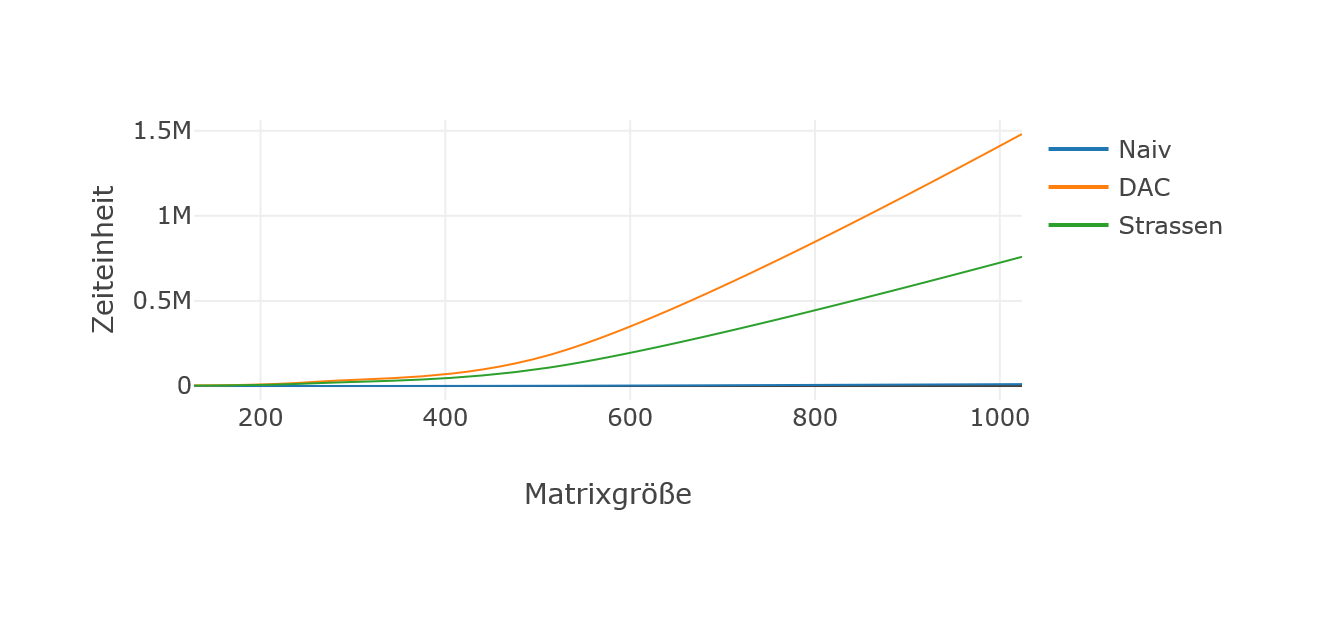
\includegraphics[width=\linewidth]{basisfallnot.png}
            \caption{Basisfall n = 1}
        \end{figure}
    }{
        \begin{figure}[H]
            \centering
            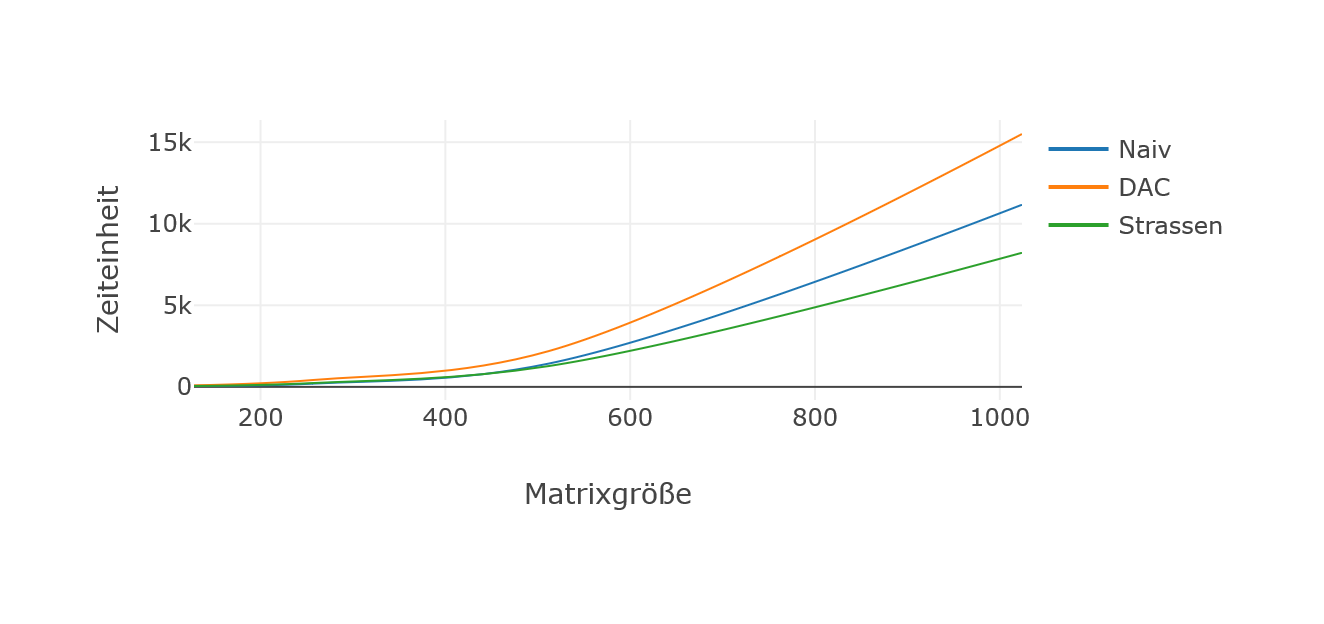
\includegraphics[width=\linewidth]{basisfallmod.png}
            \caption{Basisfall n = 32}
        \end{figure}
    }
    \pause[2]
\end{frame}

\begin{frame}{Behandelnde Algorithmen}
    In diesem Vortrag zu behandelnde Algorithmen:
    \begin{itemize}
        \item \st{Der "naive" Algorithmus}
        \begin{itemize}
            \item $\Theta(n^3)$
        \end{itemize}
        \item \st{Divide-And-Conquer-Algorithmus}
        \begin{itemize}
            \item $\Theta(n^3)$
        \end{itemize}
        \item \st{Strassens Algorithmus}
        \begin{itemize}
            \item $\Theta(n^{2,81})$
        \end{itemize}
    \end{itemize}
\end{frame}

\section{Ausblick}
\begin{frame}{Ausblick}
    $\rightarrow$ Für allgemeine Matrizen:
    
    \qquad $\rightharpoonup$ Matrizen vergrößern auf nächstgrößeres $2^k \times 2^k$
    
    \qquad $\rightharpoonup$ Fälle modifizieren
    
    \bigskip
    $\rightarrow$ Basisfall auf bestimmtes "Crossover" festlegen
    
    \bigskip
    $\rightarrow$ Parallelismus machbar
    
    \bigskip
    $\rightarrow$ Coppersmith und Winograd in $O(n^{2,376})$ \cite{10.5555/1614191}
    
    \bigskip
    $\rightarrow$ Algorithmus mit weniger als 7 Produkte existiert nicht \cite{https://doi.org/10.48550/arxiv.math/0407224}
\end{frame}

\section{Literatur}
\begin{frame}{Literatur}
    \nocite{*}
    \bibliographystyle{plain}
    \bibliography{sem.bib}
\end{frame}

\end{document}